\section{Detekcja i przeciwdziałanie kolizjom}
\label{ch:alg-collision-avoid}
Do zademonstrowania prostego przeciwdziałania kolizjom robotów wykorzystano metodę LRA* ({\it Local-Repair A*}).
W rozdziale tym opisano własną implementację tej metody.
Należy zaznaczyć, że jest to bardzo uproszczone podejście i stanowi wstęp do bardziej złożonego algorytmu.
Dużo skuteczniejsza w zapobieganiu kolizji jesto metoda WHCA* (por. \ref{ch:alg-whca}) z dynamicznym przydziałem priorytetów (por. \ref{ch:alg-priorities-allocation}), która została opisana w późniejszych rozdziałach.

Przez kolizję będziemy rozumieć sytuację, w której przynajmniej 2 roboty przebywają w tym samym miejscu (na tym samym polu) i w tym samym czasie (w tym samym kroku czasowym). Warto dodać, że dopuszczalne jest przecinanie się trajektorii robotów w różnym czasie.

Zasada działania LRA* mocno opiera się na standardowym algorytmie A*. Usprawnieniem jest wykonywanie korekcji tras w przypadku lokalnie wykrytych kolizji.

Planowanie trajektorii odbywa się dla każdego agenta niezależnie, stosując algorytm A*. Przy wyznaczaniu najkrótszej drogi uwzględniane są (jako zajęte pola) zarówno wszystkie przeszkody statyczne, jak i aktualne pozycje pozostałych robotów. Wyznaczona ścieżka dzielona jest na pojedyncze akcje agenta (ruchy robota), które zostają zakolejkowane na liście akcji do wykonania przez robota. Jeśli droga do celu nie mogła zostać wyznaczona, próba ta zostaje powtórzona w następnym kroku.

W każdym kroku symulacji agenci poruszają się wzdłuż wyznaczonych tras. Co prawda w kolejnych krokach ścieżki te mogą być już nieaktualne, jednak agenci wciąż nimi podążają, aż do osiągnięcia punktu docelowego lub wykrycia kolizji.
Wykrycie kolizji w tym przypadku nie oznacza odnotowania faktycznego zderzenia (przebywania więcej niż jednego robota na tym samym polu), lecz detekcję wystąpienia takiej niepożądanej sytuacji w następnym kroku symulacji.

Detekcja potencjalnej kolizji sprowadza się do przeanalizowania dla każdego robota jego zaplanowanego położenia z następnego kroku. Jeśli robot nie ma zaplanowanej żadnej ścieżki, oznacza to, że jego położenie w następnym kroku będzie takie samo, jak w obecnym. Uznaje się, że kolizja może wystapić w dwóch przypadkach:
\begin{itemize}
	\item w przypadku, gdy zaplanowane położenie robota w następnym kroku jest takie samo, jak aktualne położenie innego robota;
	\item w przypadku, gdy zaplanowane położenie robota w następnym kroku jest takie samo, jak zaplanowane położenie innego robota w następnym kroku.
\end{itemize}
Sprawdzenie obu tych przypadków jednocześnie jest konieczne, aby wykrywać także zderzenia czołowe robotów zmierzających w przeciwnych kierunkach.

% TODO screen ze zderzenia czołowego

Skutkiem tak wykrytej potencjalnej kolizji jest wykonanie ponownego planowania (tylko dla jednego robota lub dla wielu) trajektorii. Uwzględnienie aktualnego położenia sąsiadującego robota zapobiega zderzeniu się z nim, gdyż pole, które on zajmuje jest już podczas ponownego planowania rozpatrywane jako nieprzejezdne.

Przy takim podejściu priorytety robotów nie mają znaczenia, zaś samo planowanie może odbywać się dla agentów równolegle.
W celu poprawy wydajności technikę tą można połączyć z algorytmem D* Lite, D* Extra Lite lub RRA*.

Łatwo zauważyć, że metoda ta nie zapobiega tworzeniu się cykli planowanych akcji - powtarzających się w nieskończoność sekwencji tych samych ruchów, nie doprowadzają agentów do celów (por. rys. \ref{fig:robopath-lra-cycle}).

\begin{figure}
	\centering
		\subfloat[]{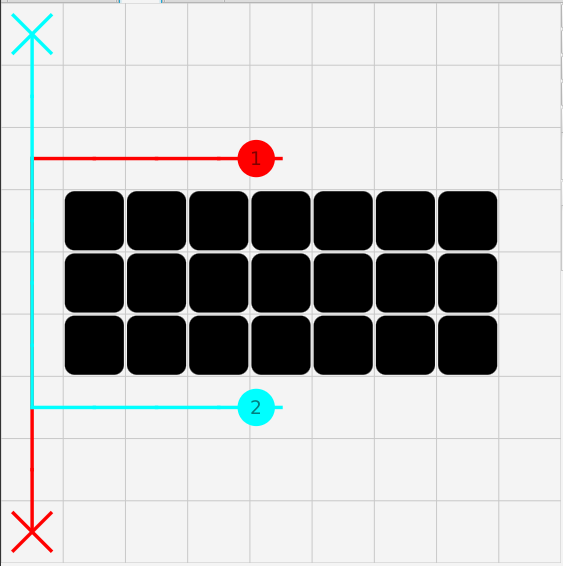
\includegraphics[width=0.4\columnwidth]{img/robopath/lra-cycle-1}}
		\qquad
		\subfloat[]{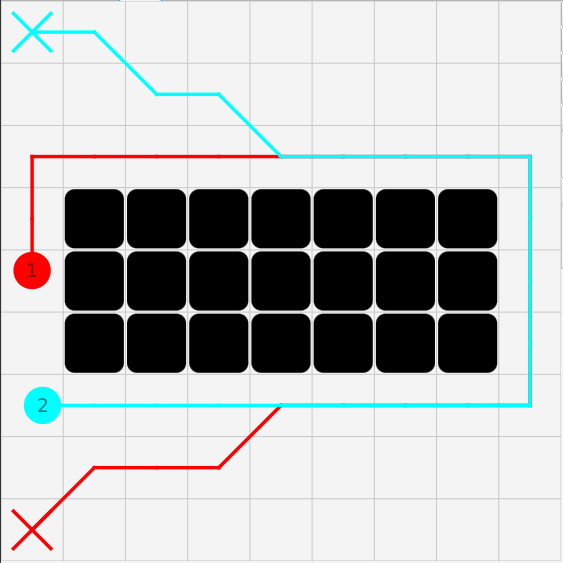
\includegraphics[width=0.4\columnwidth]{img/robopath/lra-cycle-2}}
	\caption{Przykład układu z powtarzająm się cyklem akcji planowanych przez metodę LRA*:
	(a) Dwa roboty wyznaczają niezależnie drogi do swoich celów.
	(b) Chcąc uniknąć zderzenia w wąskim przejściu po lewej stronie, roboty wyznaczą trajektorie przechodzące przez alternatywną ścieżkę po prawej stronie, gdzie ponownie dojdzie do przecięcia się trajektorii.}
	\label{fig:robopath-lra-cycle}
\end{figure}


% $TODO$ screeny ciekawych przypadków
\begin{figure}
	\centering
	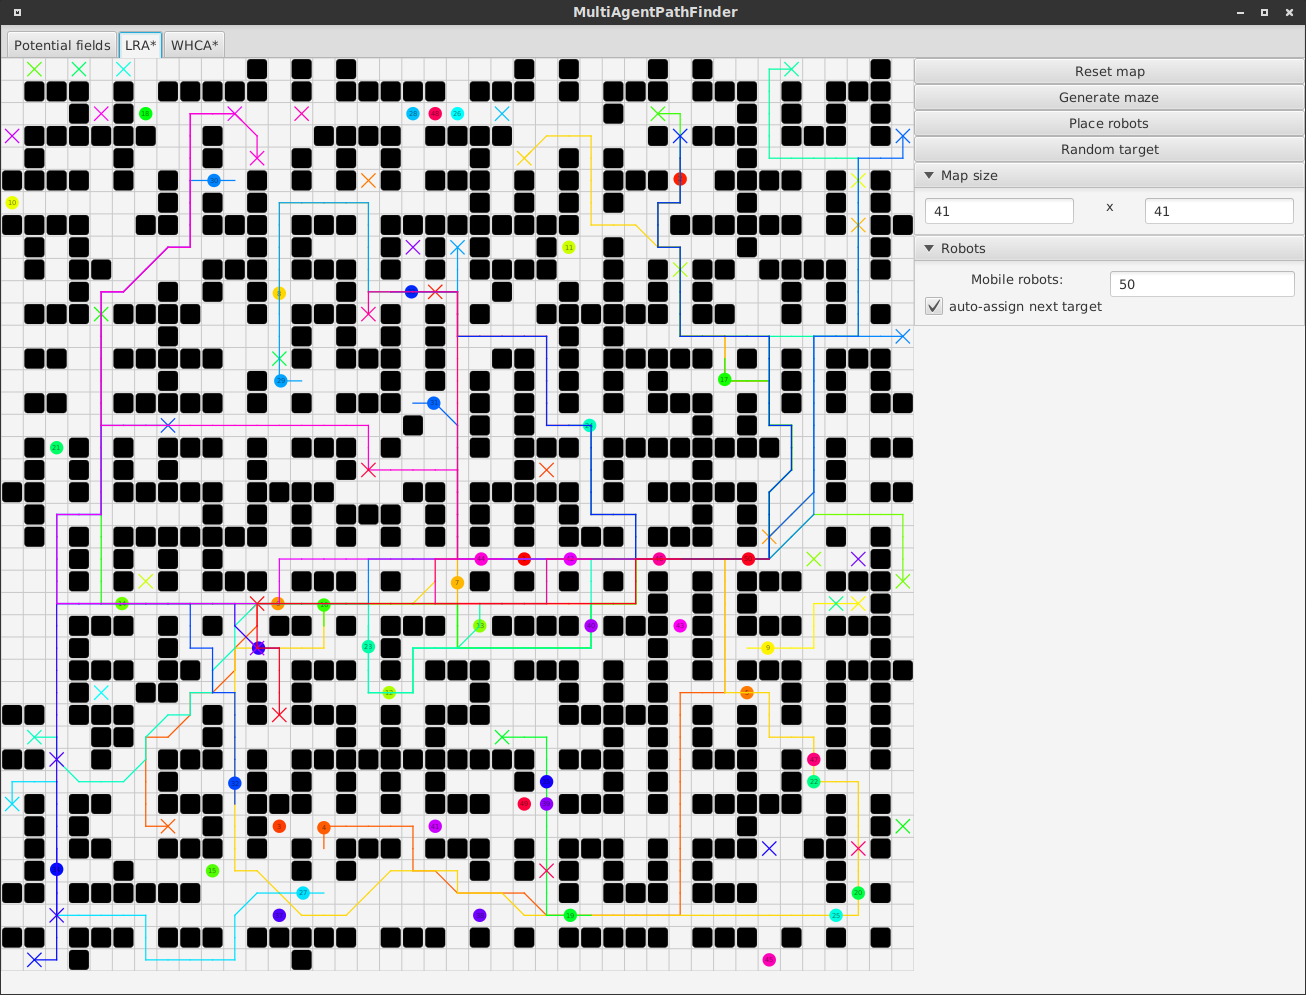
\includegraphics[width=0.8\columnwidth]{img/robopath/lra-bigmap}
	\caption{Przykład symulacji ruchu robotów metodą LRA* na dużej mapie z dużą liczbą robotów}
	\label{fig:test-lra-bigmap}
\end{figure}

% \begin{figure}
% 	\centering
% 	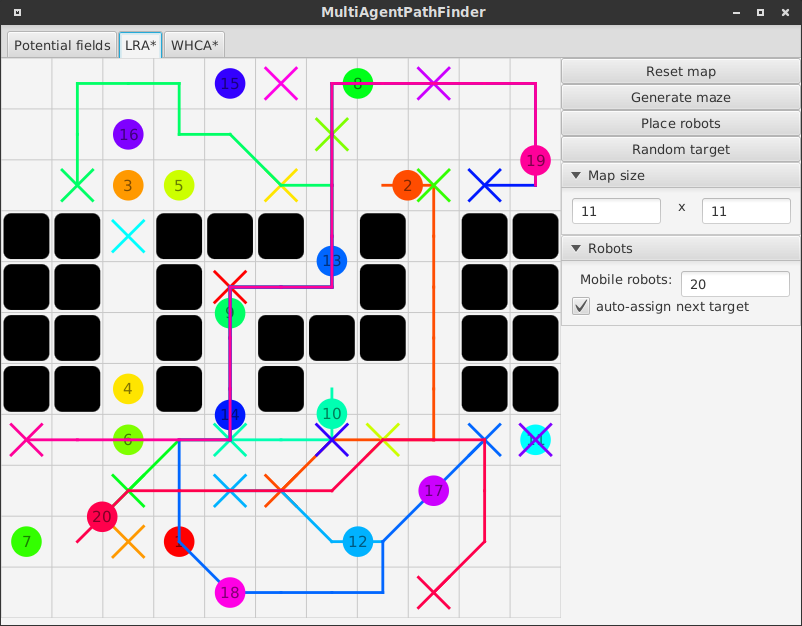
\includegraphics[width=0.8\columnwidth]{img/robopath/lra-lot-robots}
% 	\caption{Metoda LRA*: dużo robotów, mała mapa}
% 	\label{fig:test-lra-lot-robots}
% \end{figure}